\chapter{Simulation tests} %Preliminary Results
The intil phase of this project involved simulating beam dumping of the proposed electron beam of the EuPRAXIA project. This is a EU-funded project involving XXX nations and XXX insitutions. The ultimate aim is to create a compact 5 GeV laser-driven plasma wakefield accelerator for electrons, combined with an undulator to generate high-quality x-rays for research and medicine. Currently the studies are concerned with generating a high-quality 1 GeV electron beam. As the simulations and experiments yield successful results the energy will be increased untill the 5 GeV goal is reached. The electron beam parameters for this beam are given in table \ref{eupraxia_parameters}, where case 1 and 2 represents expected electron beam results for laser-driven and beam driven accelerators respectively.  In addition, the parameters for our 1 GeV simulations are also shown. These have been chosen so as to represent expected achievable values for both cases [eupraxia2020]. 
\begin{table}[ht!]
\centering
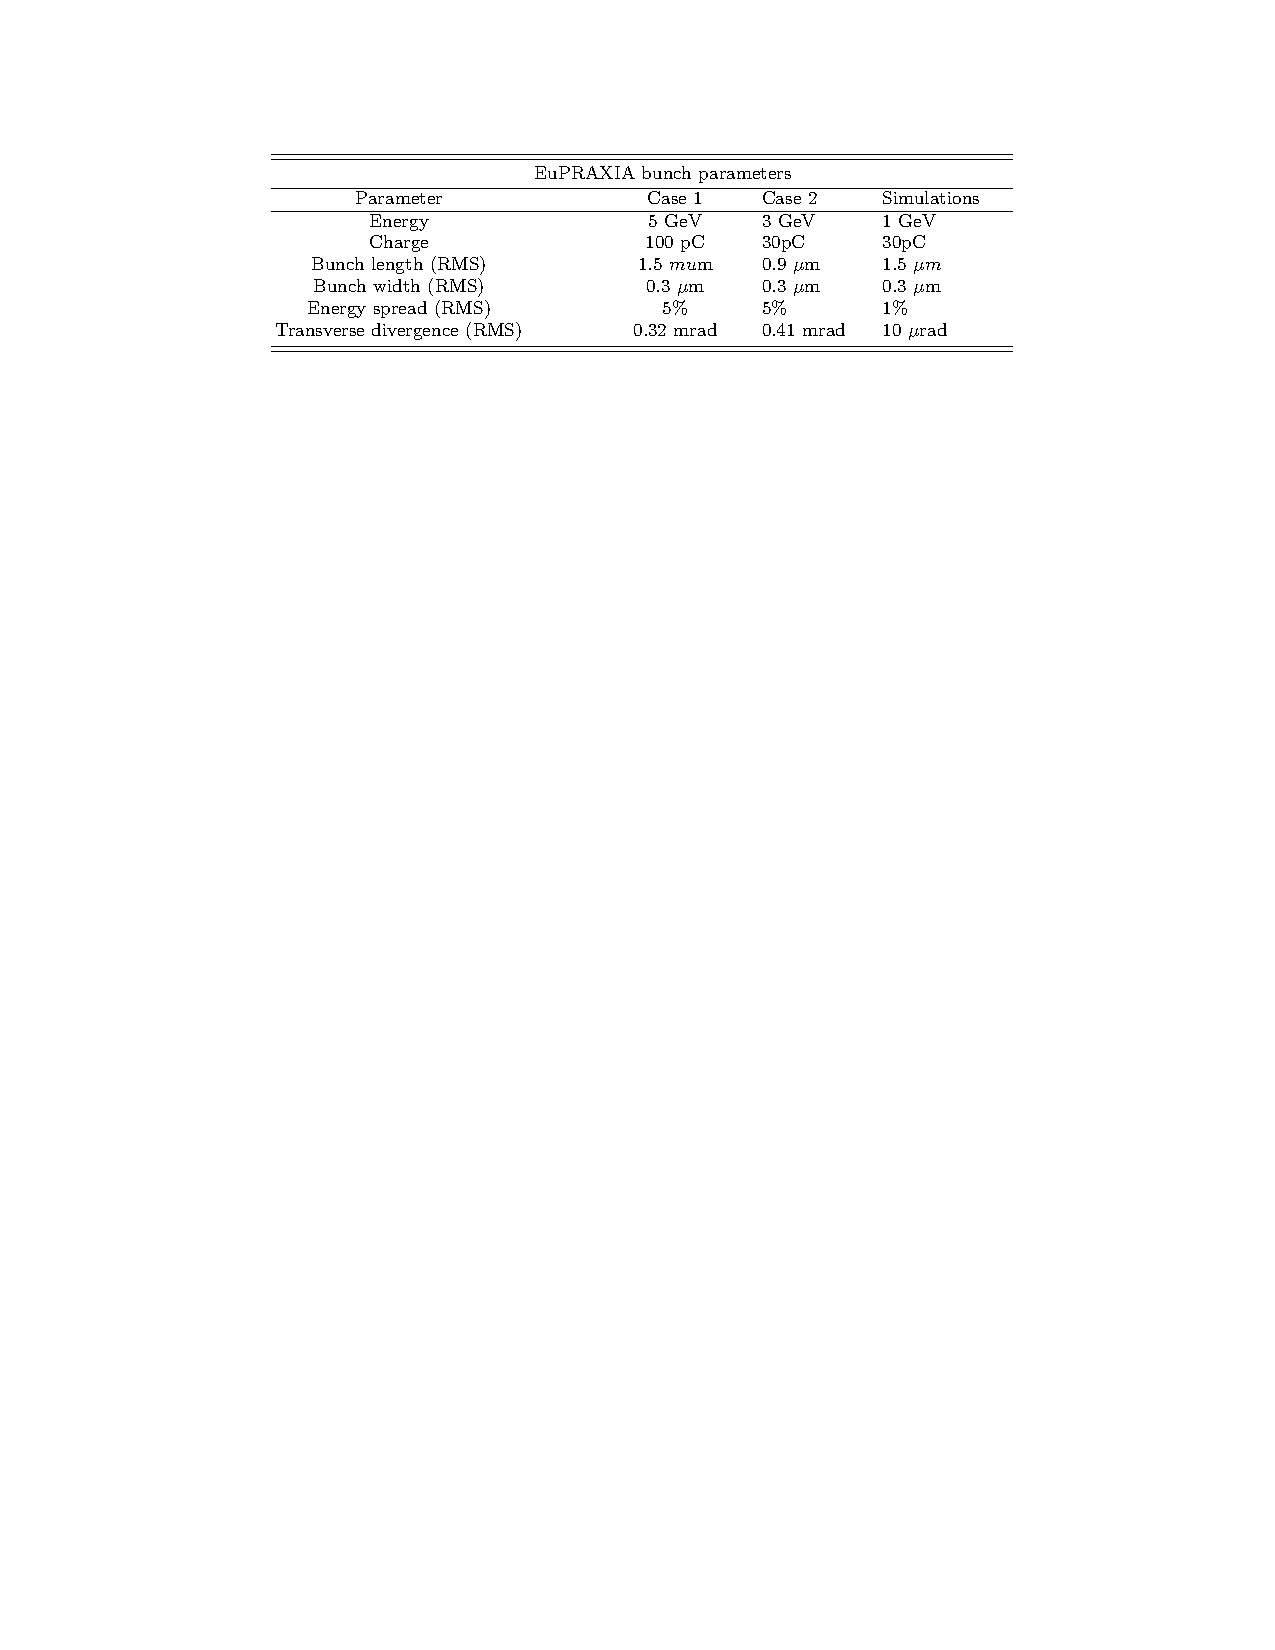
\includegraphics[width=0.8\textwidth]{table.pdf}
\caption{Parameters for the electron bunch in the EuPRAXIA project.}
\label{eupraxia_parameters}
\end{table}
\section{Plasma deceleration - Uniform density}
The EuPRAXIA project endeavours to explore what is achieve in a compact plasma wakefield accelerator with current and expected future technologies. For this reason it is interesting to explore the beam dumping quality that the current plasma technologies can achieve. Working with the simualtion beam in table \ref{eupraxia_parameters} we know from equations \ref{energy_loss_bonatto} and \ref{longitudinalforce} that the shortest beam dumping distance is achieved with the highest possible plasma density, provided that the beam is contained within the decelerating region as shown in figure \ref{theory_vs_simulation}. Most plasma wakefiled experiemnts use plasma densities $<10^18 \text{cm}^{-3}$ [ref...]. These are achieved using plasma discharge tubes.... These can provide highly uniform plasmas over several meters.\\
Higher densities, up to $<10^20 \text{cm}^{-3}$, are however achievable using supersonic gas jets \cite{Schmid2012}. This technique forces gas through a thin nozzel from a high-pressure region into a vacuum container creating a high-density gas jet. This jet can then be ionised using a laser to generated the desired high-density plasma. Currently these techniques are used to generate plasmas up to a centimetre in length. The result of letting our 1 GeV electron bunch propagate through a plasma of $10^20 \text{cm}^{-3}$ is shown in figures 1a-c. These show the average energy of particles with respect to their position in the bunch.  
\section{Larger bunch}
using more realistic bunch parameters we here present two simulations. 

\begin{figure}
\centering
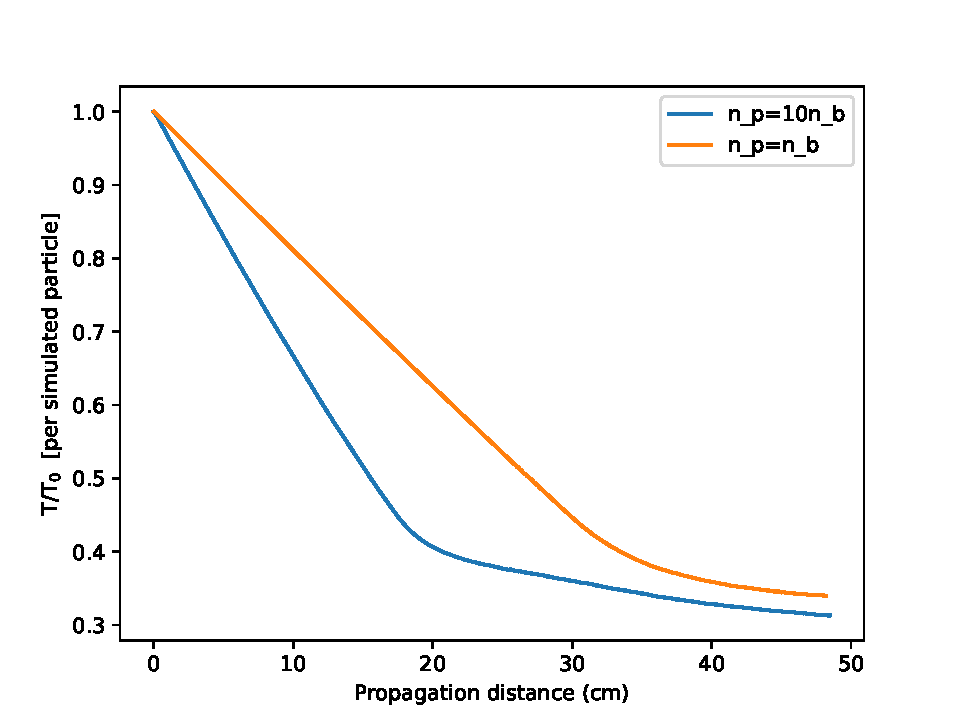
\includegraphics[width=0.8\textwidth]{Energy30pc_per_particle_lowres.pdf}
\caption{•}
\end{figure}

\begin{figure}
\centering
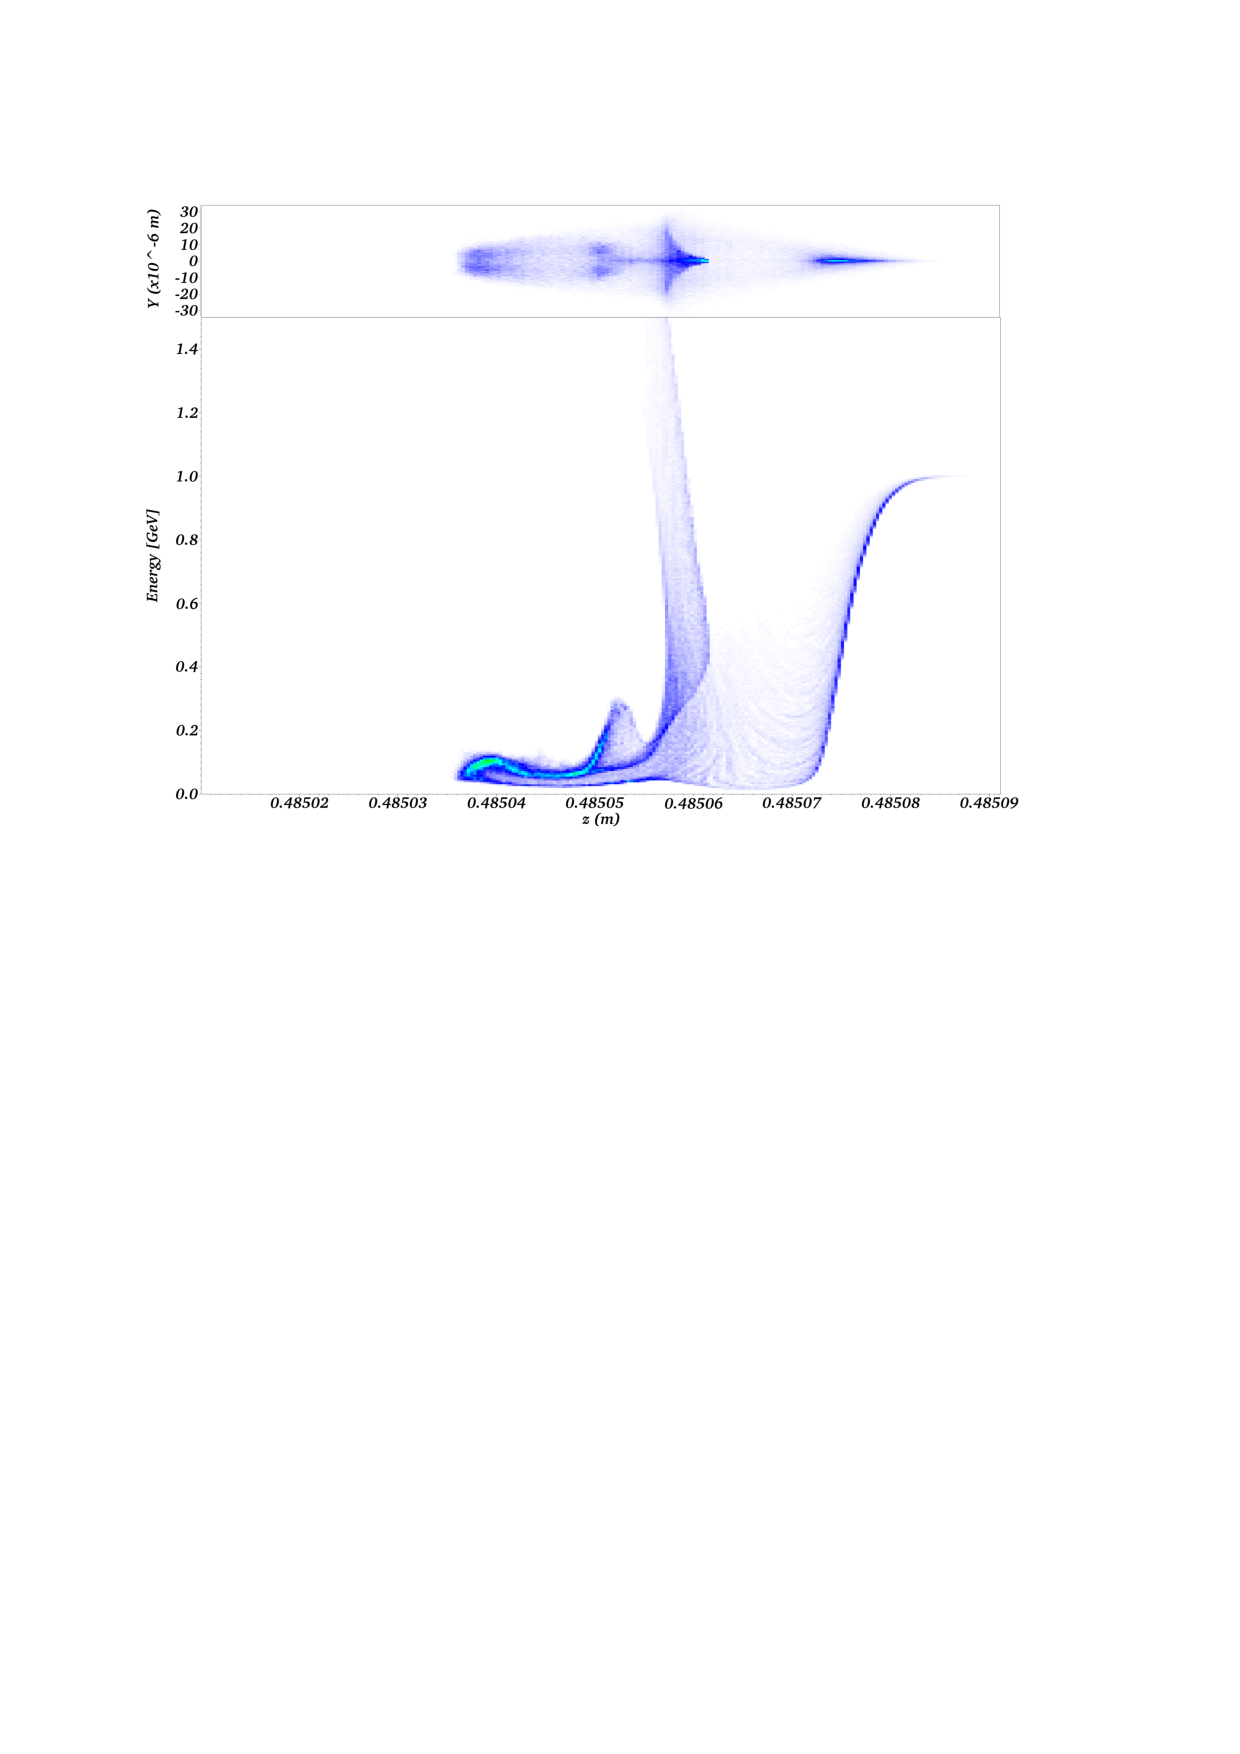
\includegraphics[width=0.85\textwidth]{bunch_and_energy_48cm.pdf}
\end{figure}
\subsection{Transverse instabilities in quasilinear regime}
\begin{figure}
\centering
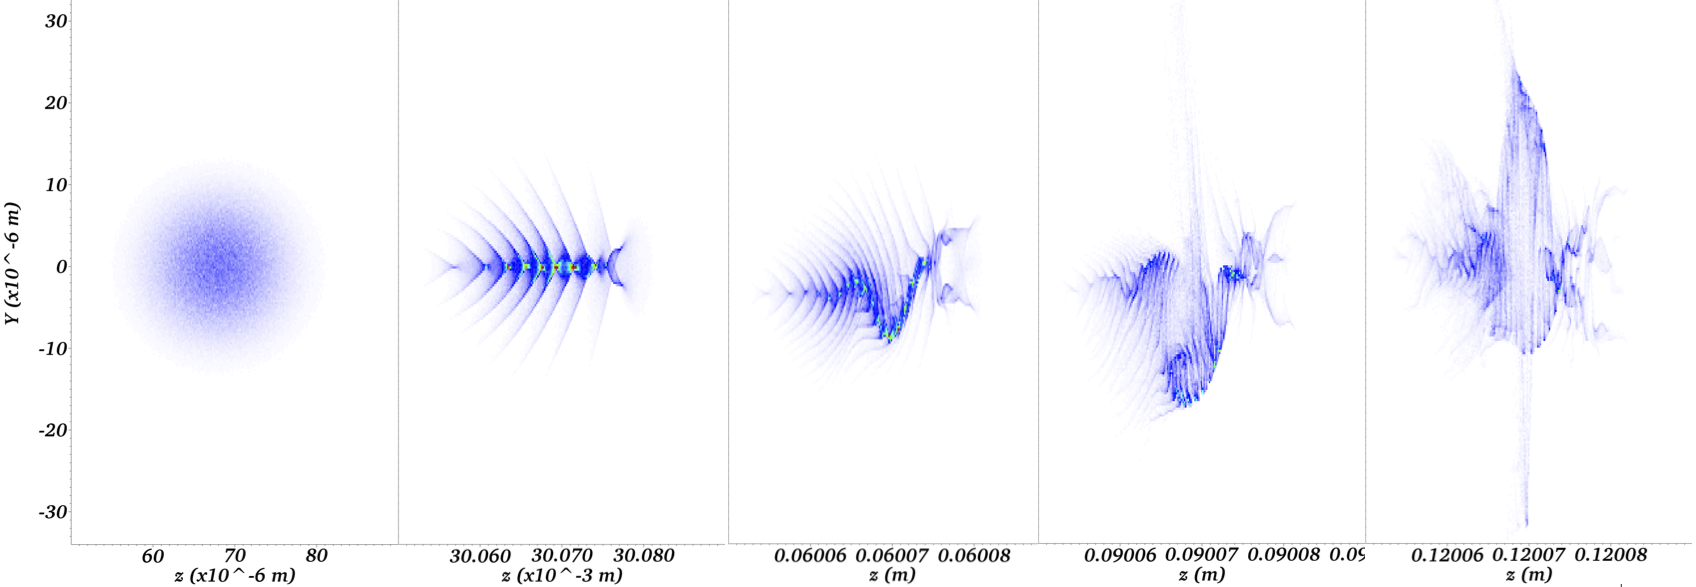
\includegraphics[width=\textwidth]{cherenkov_instability}
\end{figure}
\section{Hybrid Scheme - Feasibility study}
\subsection{Initialising a decelerated bunch}
-Compare to actual already propagated bunch we want to simulate. See how quickly the uniform plasma resembles that of the plasma of the propagated simulation. If it takes long time then the laser results might not represent the real situation.  Compare simulations side by side as both real and initialised bunches propagate further, see if any deviations occur or if the bunch I set up is actually a fair approximation (compare energy, particle number etc.)
\subsection{Introduction of co-propagating laser}
- Results with respect to laser intensity/amplitude/wavelength as well as distance from bunch.


%\clearpage
%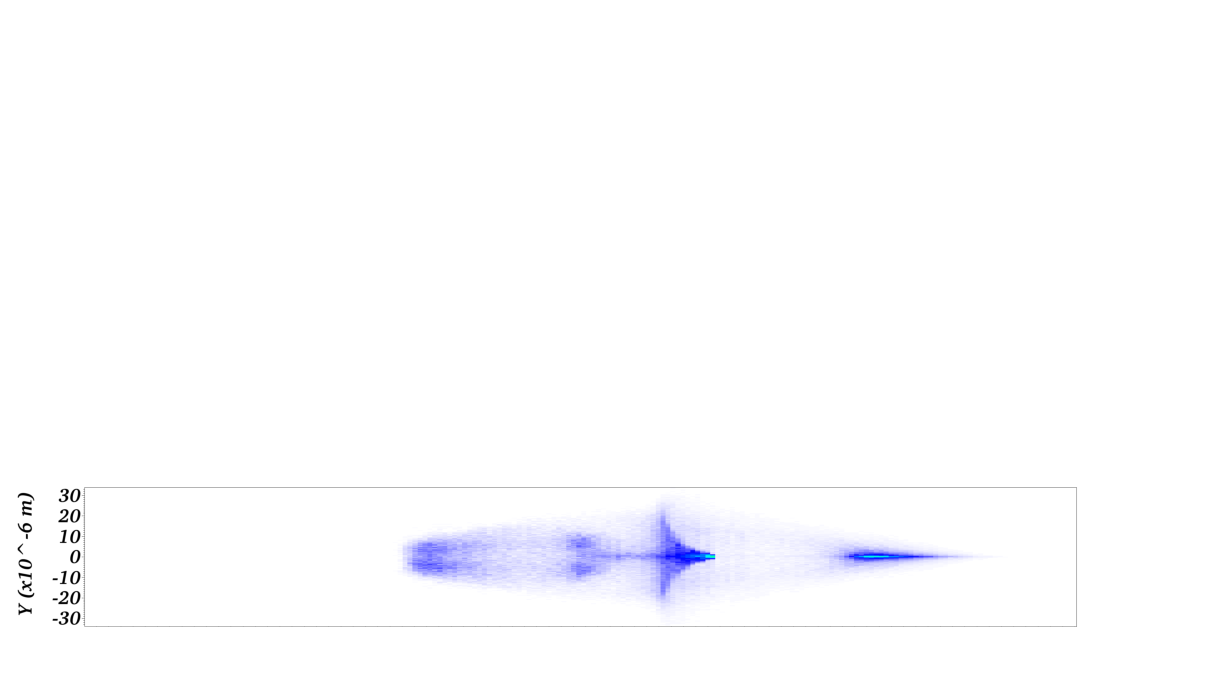
\includegraphics[width=\textwidth]{bunch_linear_48cm}\vspace{-1pt}\\
%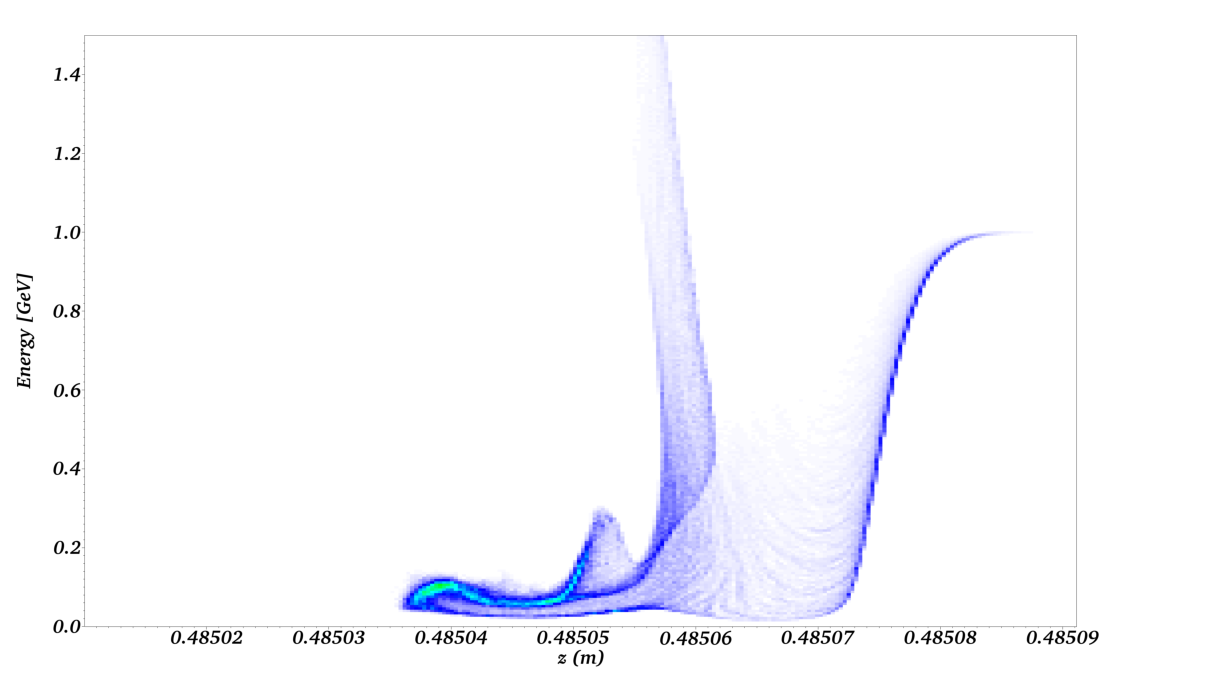
\includegraphics[width=\textwidth]{energy_linear_48cm}